\chapter{Sense Amplifier analyse}
\label{sensamp}
Een sense amplifier versterkt kleine signaalverschillen tot rail-tot-rail signalen. Aangezien de uitgangsignalen hiervan ook de uitgelezen bits zijn van het geheugen, is het bovenal belangrijk dat dit op een correcte manier gebeurt, ondanks variabiliteit.
Het is dus logisch om de sense amplifier wat meer te onderzoeken en zodanig te ontwerpen op een robuuste manier, terwijl er ook rekening gehouden wordt met energie en snelheid.

\section{Types SA}
...
\begin{figure}
  \centering
  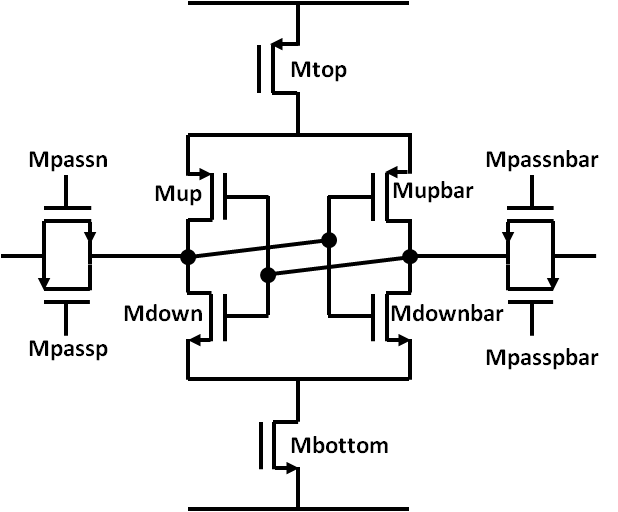
\includegraphics[scale=0.4]{../fig/hfdstk-sensamp-ourSA.png}
  \caption{een sense amplifier}
  \label{fig:ourSA}
\end{figure}

In wat volgt zal er worden voortgewerkt met de SA van figuur \ref{fig:ourSA}.


\section{Offsetspanning}
Een ideale sense amplifier zal voor elke twee ingangssignalen correct versterken, tenzij de signalen dezelfde zijn, waarna de SA in een metastabiele toestand belandt. In de praktijk is er echter wegens variabiliteit een limiet voor het ingangsspanningsverschil waarbij er correct versterkt wordt. Deze limiet heet de offsetspanning en wordt geïllustreerd in figuur \ref{fig:offset}. De offsetspanning van een SA is in de ontwerpfase een stochastische variabele met gemiddelde 0V, pas nadat een chip gefabriceerd is ligt de offsetspanning definitief vast [al kan het zijn dat deze met de tijd nog verandert].
Er zijn 2 manieren waarop men de offsetspanning van een systeem kan aanpakken: ofwel ontwerp je het systeem zodanig dat het verschil van de ingangssignalen van de SA groot genoeg is zodat ze [in 99,9\% van de gevallen] niet groter is dan de offsetspanning, ofwel bouw je een mechanisme in waarbij je na fabricatie de offsetspanning meet en vervolgens compenseert. In dit werk is gekozen voor het eerste.
Hiervoor is het wel belangrijk te onderzoeken wat de verdeling is van de offsetspanning, dit wordt gedaan in de volgende sectie.

\begin{figure}
  \centering
  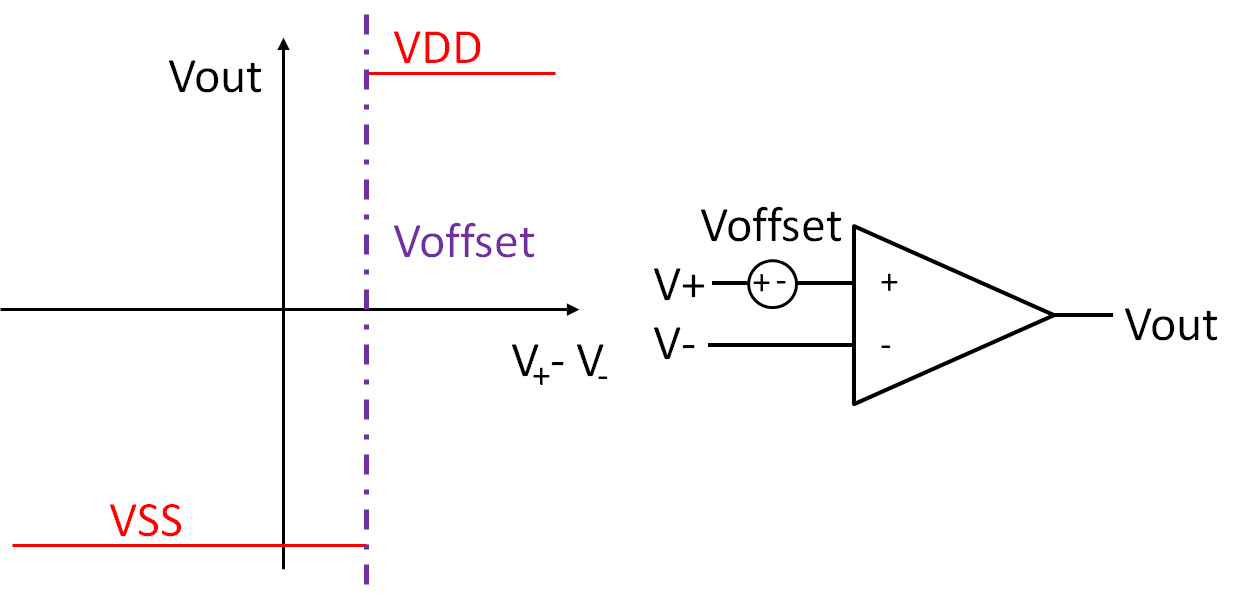
\includegraphics[scale=0.4]{../fig/hfdstk-sensamp-offset.png}
  \caption{Illustratie van offsetspanning}
  \label{fig:offset}
\end{figure}

\section{Sensitiviteitsanalyse}
De SA wordt gerealiseerd als een circuit met transistors. Elke transistor heeft 2 stochastische parameters met een normale verdeling, nl. $\Delta V\textsubscript{t}$ en $\Delta \beta$. De spreiding van deze verdelingen is gekend: $\sigma_{\Delta V_{t}} = \frac{A\textsubscript{V\textsubscript{t}}}{\sqrt{W L}}$ en $\sigma_\frac{{\Delta \beta}}{\beta} = \frac{A_{\beta}}{\sqrt{W L}}$. Met een sensitiveitsanalyse kan men uit deze standaardafwijkingen de standaardafwijking van de offsetspanning $\sigma_{V_{offset}}$ berekenen. Hierbij wordt verondersteld dat de stochastische variabele $V_{offset}$ een lineaire combinatie is van de normaal verdeelde afwijkingen $(\Delta V_{t})_{i}$ en $(\frac{\Delta_{\beta}}{\beta})_{i}$: $V_{offset}=\sum\limits_{i=1}^{N} a_{i} (\Delta V_{t})_{i} + b_{i} (\frac{\Delta_{\beta}}{\beta})_{i}$.
$a_{i}$ en $b_{i}$ zijn de gevoeligheden van de offset naar de variatieparameters: $a_{i}=\frac{\partial V_{offset}}{\partial (\Delta V_{t})_{i}}$ en $b_{i}=\frac{\partial V_{offset}}{\partial (\frac{\Delta_{\beta}}{\beta})_{i}}$.
Voor een dergelijke variabele geldt dan: $\sigma_{V_{offset}}=\sqrt{\sum\limits_{i=1}^{N} a_{i}^{2} (\sigma_{\Delta V_{t}})_{i}^{2} + b_{i}^{2} (\sigma_{\frac{\Delta_{\beta}}{\beta}})_{i}^{2}}$.

Er moet wel geverifieerd worden of de stelling dat er een lineaire afhankelijkheid is tussen $V_{offset}$ en de variatieparameters gegrond is.
Dit kan gedaan worden aan de hand van een analyse waarbij elke variatieparameter afzonderlijk gesweept wordt. 
In figuur \ref{fig:min-sensanalysis} wordt het resultaat getoond voor een dergelijke analyse bij een SA met minimale afmetingen, in tabel \ref{tab:min-sensanalysis} worden de resultaten en de resulterende standaardvariatie van de SA getoond.
Er moet opgemerkt worden dat er bij deze simulatie slechts gesweept werd voor de variatieparameters van -4$\sigma$ tot 4 $\sigma$. Dit is om de reden dat voor de minimale transistoren de standaardvariatie het grootst is. In de Spectre-simulaties zouden transistoren voor te grote negatieve $\beta$-mismatch stroom leveren in de omgekeerde richting. Deze situatie zal fysisch nooit optreden.

Opmerkelijk bij deze analyse is dat er een significante bijdrage is van de pass-gates door $\beta$-mismatch. Een nadere observatie leert dat deze bijdrage optreedt door ladingsinjectie van de pass-gates die niet meer gematched is (zie figuur \ref{fig:chargeinjectionmismatch}).
Hierbij moet wel worden opgemerkt dat voor deze simulatie er geen overlap is tussen het controlesignaal op de passgate aan te zetten en het signaal om de SA te activeren.
De reden hierachter is dat als er overlap tussen deze signalen is, de SA ook de BL zou trachten op te laden. Hierbij zou er moeten ingeboet worden aan snelheid en het zou ook extra energie kosten.

Men kan argumenteren dat er een korte overlap zou kunnen toegelaten zijn, waarna er voldoende spanningsverschil tussen de 2 ingangs-uitgangsknopen zou opgebouwd zijn opdat de ladingsinjectie geen effect meer kan hebben op het eindresultaat. Een tegenargument is dat de timing hiervoor te precies moet zijn.
\begin{figure}
  \centering
  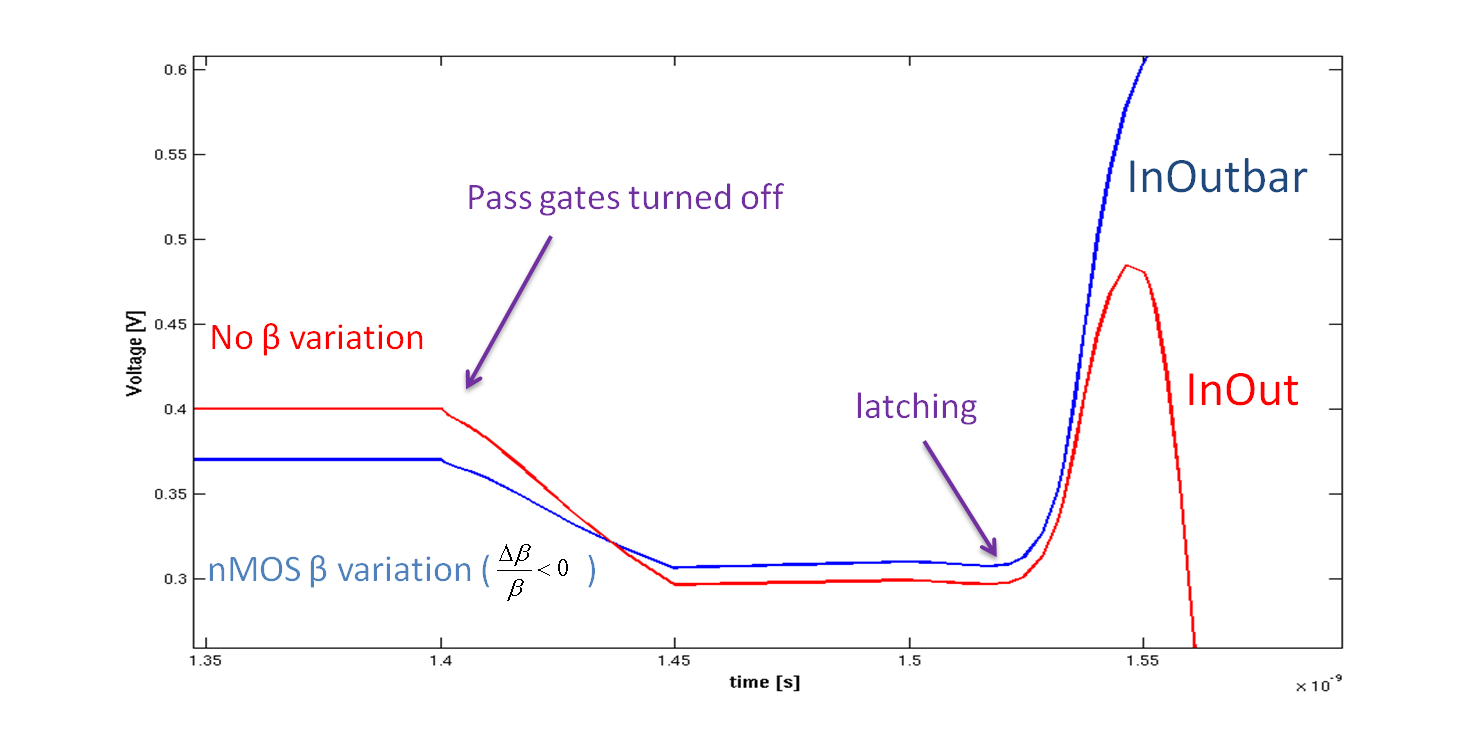
\includegraphics[scale=0.4]{../fig/hfdstk-sensamp-chargeinjectionmismatch.png}
  \caption{Door $\beta$-mismatch is ladingsinjectie van de pass-gates niet meer gematched en gaat de SA foutief latchen}
  \label{fig:chargeinjectionmismatch}
\end{figure}

\subsection{RC-latch-effect}
De situatie waarbij er volledige overlap is tussen de controle signalen kan vereenvoudigd worden opgesteld met de situatie van figuur \ref{fig:RC-latch}. De pass-gate die aanstaat wordt voorgesteld als een weerstand, de pass-gate in het local block en diens parasitaire capaciteit wordt verwaarloosd. CL bedraagt voor deze simulatie 46 fF, het equivalent voor een BL waaraan 256 cellen hangen. Cint bedraagt voor een SA met minimale transistorafmetingen 161 aF. Wanneer het dynamisch latch-gedrag bekeken wordt voor verschillende waardes van R, treedt er een merkwaardig effect op (zie figuur \ref{fig:RC-latch-sim}): voor voldoende grote waardes van R lijkt het alsof de grote capaciteit ontkoppeld is van de latch tot op een zeker tijdstip, waarna een veel tragere settling optreedt.
De verklaring ligt in het feit dat CL zich voor hoge frequenties als een kortsluiting gedraagt (zie figuur \ref{fig:RC-latch-explain}), een plotse stroom vloeit door de weerstand en hierdoor onstaat er een spanningsval over de weerstand. Hierna gaat er op veel lagere frequenties een spanning beginnen vormen over de capaciteit waardoor de ingangs-uitgansknopen volledig kunnen laden/ontladen tot VDD en VSS.

\begin{figure}
  \centering
  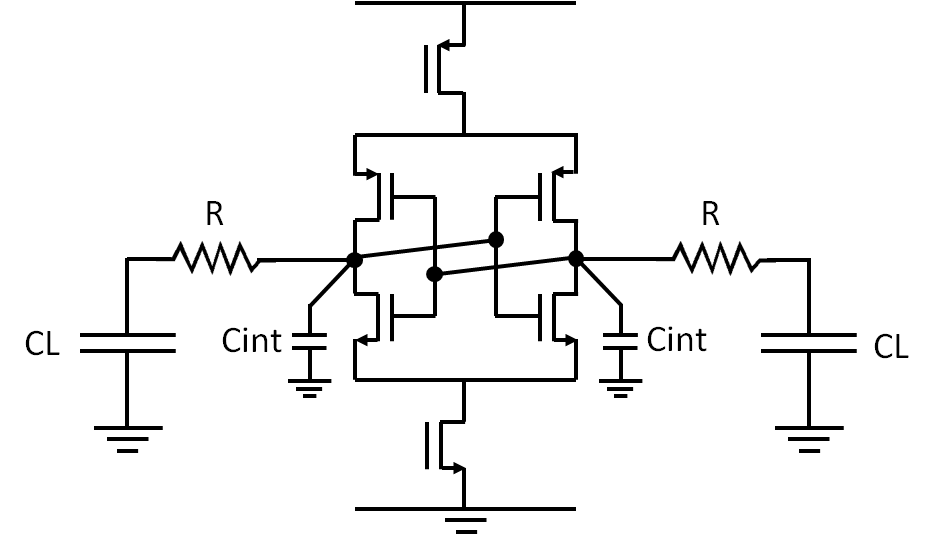
\includegraphics[scale=0.4]{../fig/hfdstk-sensamp-RC-latch.png}
  \caption{Simulatieopstelling voor het RC-latch-effect}
  \label{fig:RC-latch}
\end{figure}

\begin{figure}
  \centering
  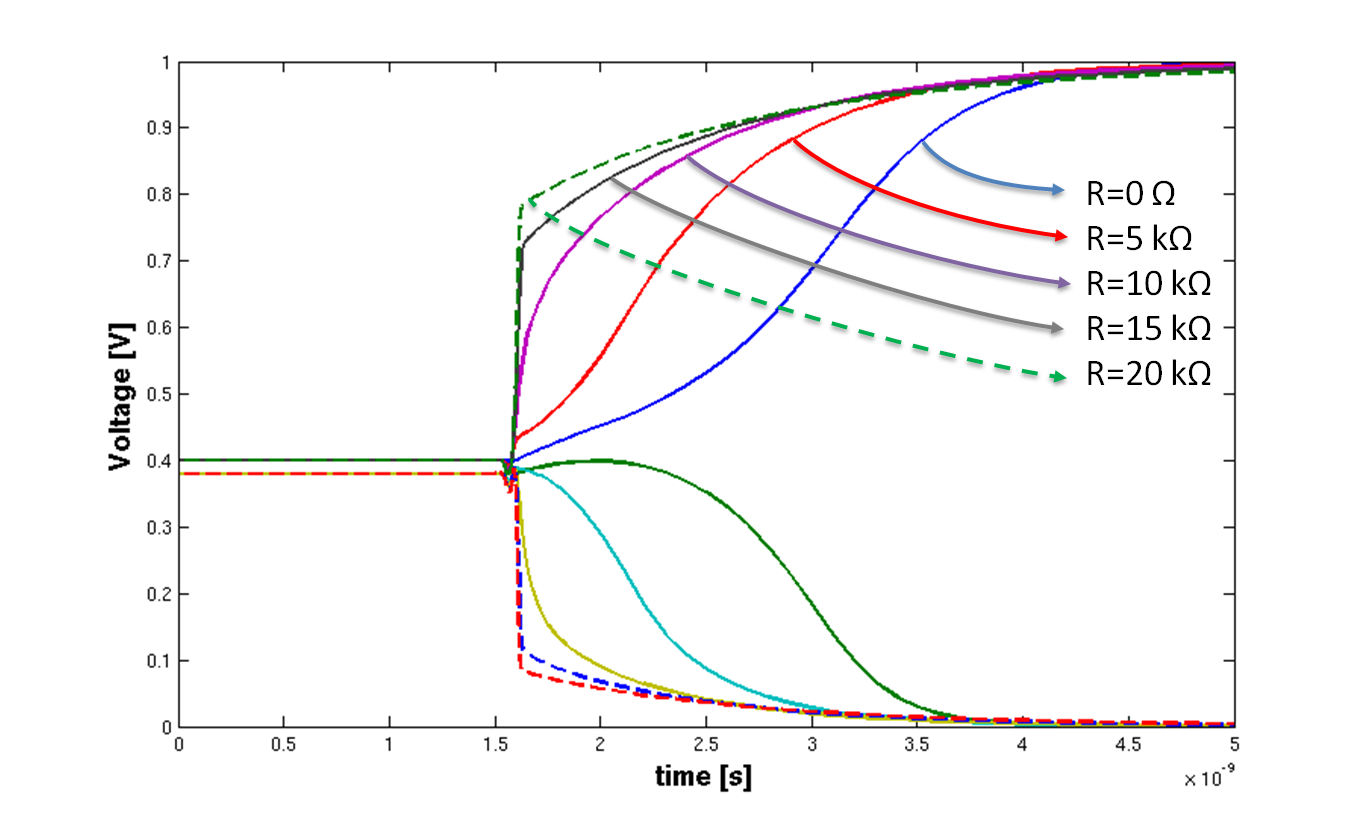
\includegraphics[scale=0.4]{../fig/hfdstk-sensamp-RC-latch-sim.png}
  \caption{Simulatieresultaten voor het RC-latch-effect:de 2 ingangs-uitgangsknopen zijn voorgeladen op 400mV en 380mV. Na 1,6ns wordt de SA aangezet. De SA is ideaal voor deze simulatie.}
  \label{fig:RC-latch-sim}
\end{figure}

\begin{figure}
  \centering
  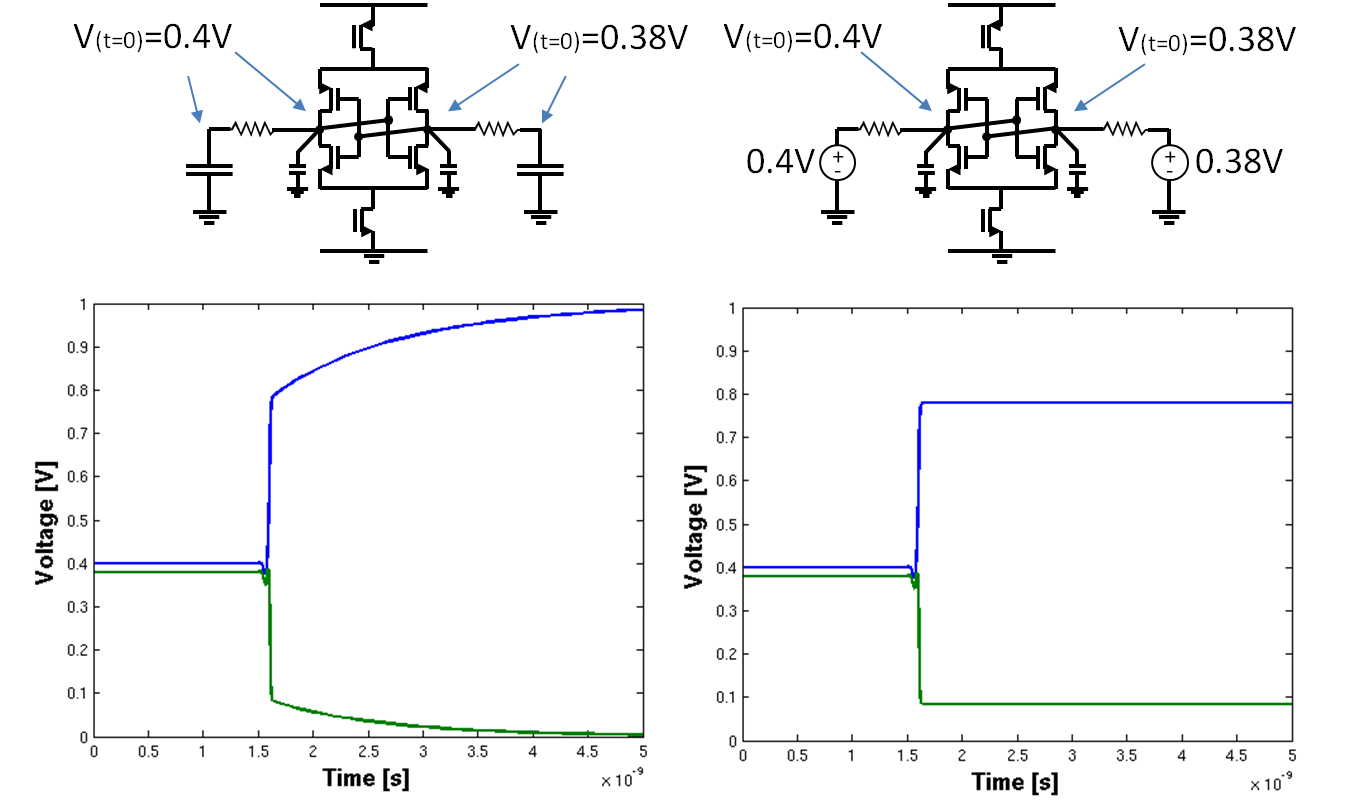
\includegraphics[width=\textwidth]{../fig/hfdstk-sensamp-RC-latch-explain.png}
  \caption{Vergelijking situatie met voorgeladen (eindige) capaciteit en situatie met spanningsbron (oneindige capaciteit)}
  \label{fig:RC-latch-explain}
\end{figure}

\section{Paretosimulatie}



\section{Besluit}
